\chapter{The Power of Cameos}
\label{ch:cameos}
\index{cameos}
\index{character presence}

\begin{chapterabstract}
This chapter explores the transformative power of character presence in AI-generated video, examining how ``cameos'' function as narrative anchors that elevate abstract imagery into emotionally resonant storytelling. We define three primary cameo types: named cameos using the @mention system for identity consistency, descriptive cameos constructed through detailed textual characterization, and conceptual cameos that transform abstract ideas into visual metaphors. The chapter addresses the profound experience of self-entrance—when creators appear in their own AI-generated content—and its implications for personal narrative and identity exploration. We examine practical techniques for directing character performance through language, including posture control, emotional expression, and interaction dynamics. Ethical considerations receive substantial attention, covering consent requirements, likeness rights, cultural sensitivity, and the responsible use of real-world identity representation. The chapter also explores brand cameos for commercial applications, demonstrating how corporate identity can be embodied through character presence. By understanding cameos as narrative consciousness rather than mere visual elements, readers gain sophisticated tools for creating compelling character-driven AI films.
\end{chapterabstract}

When you first opened Sora 2, perhaps out of mere curiosity, you typed a few descriptive phrases and watched as it transformed words into light and shadow, sentences into scenes. In that moment, what you experienced was the technical capability of AI video generation—a visual sequence created from your textual input. Yet true cinematic language doesn't reside in landscapes and architecture, but in \textit{people}\index{human element}. The first time you bring a specific person into the frame—even if it's just a blurred silhouette, a breath, a sigh—your imagery begins to acquire emotional resonance. It transforms from abstract visual content into compelling human narrative.

The ``cameo''\index{cameo} is the core switch of this transformation. It's a form of \textbf{narrative invocation}\index{narrative invocation}, enabling abstract imagery to resonate with audience emotions. It transforms AI-generated worlds from cold to warm, from meaningless to meaningful. Whether it's yourself, a fictional character, a brand representative, or the symbolic projection of a historical figure, their appearance grants the story temporal depth and psychological dimension. This chapter will guide you through a systematic understanding of the power of cameos—from textual commands to shot composition, from ethical boundaries to brand narratives, from concrete performance to spiritual symbolism. You'll learn how to use precise language commands to direct character performance and create compelling narratives in AI-generated video.

\section{What is a ``Cameo'': Character Integration and Narrative Structure}
\label{sec:cameo-definition}
\index{cameo!definition}

In Sora 2's semantic system\index{Sora 2!semantic system}, a ``cameo'' represents not merely ``someone appearing,'' but an \textbf{embedding of identity}\index{identity embedding}. When you include a named character or symbol in your Prompt, the system assigns it an appearance, actions, and inner emotions based on linguistic context. This mechanism liberates AI video from the floating state of a ``subjectless perspective,'' granting it the structure of ``the observed''—thus establishing a story.

Cameos take various forms, primarily three types:

\begin{enumerate}
\item \textbf{Named Cameo (@mention cameo)}\index{cameo!named}: Directly referencing an identity registered in the system, such as @zhiping or @mei. The system automatically recognizes their appearance and style, ensuring continuity and authenticity across multiple scenes.

\item \textbf{Descriptive Cameo (textual cameo)}\index{cameo!descriptive}: Constructing a character's identity purely through text, for example, ``a weary yet resolute middle-aged photographer slowly raises his camera.'' This approach gives creators greater interpretive space, suitable for literary narratives.

\item \textbf{Conceptual Cameo (symbolic cameo)}\index{cameo!symbolic}: When a character is no longer flesh and blood, but an abstract spiritual symbol. For example: ``a child made of light traverses through a forest of code.'' This represents an important form of AI visual poetics\index{visual poetics}—the transformation of abstract concepts into compelling visual metaphors.
\end{enumerate}

The essence of a cameo is to imbue the lens with a form of narrative consciousness\index{consciousness in cinema}. It's not merely a materialization of existence, but an ethical and emotional connection point of narrative. When you master this ability to ``deploy characters through language,'' you truly become the fusion of director and screenwriter.

\section{The Creator as Subject: Stepping into Your Own Film}
\label{sec:self-cameo}
\index{self-cameo}
\index{creator as subject}

Every Sora 2 creator experiences that mysterious moment: when they first appear in the frame. When the system generates a virtual ``you'' using your uploaded avatar, posture, or temperament, in that instant, you transform from observer to existential being. You're watching a dream starring yourself.

\begin{Prompt}
``@leon2346 walks through a library illuminated by sunset, dust dancing in the light, his shadow overlapping with a row of bookshelves.''
\end{Prompt}

\begin{figure}[H]
\centering

\includegraphics[height=\figheight]{Fig4-1.png}
\caption{Creator walking through sunlit library—self as narrative anchor \\ \authorcreated}
\label{fig:self-library}
\index{figure!self-cameo in library}
\end{figure}

You're no longer the operator of words, but the emotional source of imagery. The audience sees emotion through you, while AI understands the story through you. You've become the director and actor of the ``self-mirror.''\index{self-mirror}

This experience makes creation profound:

\begin{itemize}
\item You begin to contemplate ``Who am I in this frame?''
\item You realize your appearance, tone, and posture will be interpreted by the system as emotional symbols.
\item You learn to perform through language, without cameras or rehearsals.
\end{itemize}

But precisely because of this, you must also learn caution. The AI-generated you isn't only yourself—it's ``you as interpreted by language.'' Therefore, each appearance requires contextual consideration: Does it express genuine attitude? Could it be misread? Does it respect your own and others' emotional boundaries?

\section{Setting Up Your Cameo: A Step-by-Step Guide}
\label{sec:cameo-setup-guide}
\index{cameo!setup}
\index{cameo!recording process}

Creating a high-quality cameo is the foundation of all subsequent AI filmmaking endeavors. The process transforms you from a mere Prompt writer into a digital actor, enabling the system to generate realistic representations of your likeness and voice across countless scenarios. This section provides a comprehensive guide to the cameo creation process, from initial setup to optimization techniques \citep{openai2024cameos}.

\subsection{Initial Account Setup and Cameo Creation}
\index{cameo!account setup}

When you first create your account on the Sora app, you'll be given the option to create a cameo by recording a video with audio to verify your likeness. This initial setup is crucial—it establishes the baseline from which all future generations will be derived. The system uses this capture to understand your facial structure, expressions, voice patterns, and mannerisms.

The cameo creation process follows a structured sequence designed to capture maximum information about your appearance and voice:

\begin{enumerate}
\item \textbf{Environmental Preparation}: Position yourself in optimal lighting conditions
\item \textbf{Head Positioning}: Follow guided movements to capture different angles
\item \textbf{Voice Verification}: Read specific phrases for audio calibration
\item \textbf{Processing and Upload}: Allow system processing (typically 1 minute)
\item \textbf{Quality Review}: Assess results and retake if necessary
\end{enumerate}

\subsection{Recording Requirements and Technical Specifications}
\index{cameo!recording requirements}
\index{lighting!cameo recording}

The quality of your cameo directly impacts all subsequent video generations. Poor initial capture leads to inconsistent or unrealistic representations across all your AI-generated content.

\textbf{Lighting and Environment:}
\begin{itemize}
\item Record in varied lighting and try different light sources; lighting is by far the most common cause of low-quality cameos
\item Use natural light that creates some shadows on your face for dimensional depth
\item Ensure clean background with no filters, beauty effects, or distracting elements
\item Remove hats, tinted glasses, or anything that obscures facial features
\item Record in a quiet, non-echoey space with minimal background noise \citep{openai2024cameos}
\end{itemize}

\textbf{Framing and Positioning:}
\begin{itemize}
\item Hold the camera at eye level, arm's length away from your face
\item Keep your whole face in frame (forehead to chin, both cheeks visible)
\item Fill the frame with your face—avoid being positioned too far back
\item Center your face and maintain stability between movements
\end{itemize}

\subsection{Movement Patterns and Facial Expression Guidelines}
\index{cameo!movement patterns}
\index{facial expressions!cameo recording}

The cameo recording process requires specific movement patterns to capture your likeness from multiple angles. Based on the interface sequence, the process typically includes:

\textbf{Head Movement Sequence:}
\begin{enumerate}
\item \textbf{Initial Position}: Start with head slightly lowered (``lower your head'')
\item \textbf{Side Angles}: Turn head slowly left and right while maintaining exaggerated facial expressions
\item \textbf{Vertical Coverage}: Add slight up/down tilt to cover jawline and hairline areas
\item \textbf{Final Position}: Turn head toward right side (``turn head to the right'') for profile capture
\end{enumerate}

\textbf{Expression and Performance Guidelines:}
\begin{itemize}
\item Use exaggerated facial expressions (happy, sad, angry, confused) throughout recording
\item Talk continuously and expressively—more speech provides better voice modeling
\item Move at normal speed (not too fast or slow) to avoid motion blur
\item When showing side angles, look slightly up to include neck area
\item Maintain natural, varied expressions rather than static poses
\end{itemize}

\subsection{Voice Recording and Audio Calibration}
\index{voice recording!cameo}
\index{audio!cameo setup}

Voice capture is equally important as visual recording for creating authentic cameos. The system uses your voice patterns to generate synchronized speech in AI videos.

\textbf{Voice Recording Protocol:}
\begin{itemize}
\item When verification phrases appear (such as numbers like ``94, 47, 96''), read them exactly as written with no ad-libbing
\item Speak clearly at normal pace and volume—avoid whispering or shouting
\item Articulate with different parts of your voice by varying pitch and tone
\item Use different mouth shapes to capture full range of phonetic possibilities
\item Keep microphone 6-12 inches from your mouth without covering it
\item Ensure transcript verification matches your spoken words exactly
\end{itemize}

\subsection{Quality Optimization and Best Practices}
\index{cameo!quality optimization}
\index{best practices!cameo recording}

Creating a high-quality cameo requires attention to numerous technical and performance details:

\textbf{Do's:}
\begin{itemize}
\item Center your face and keep still between slow turns
\item Capture as much variation as possible in a 5-second vertical clip
\item Use natural lighting that creates dimensional shadows
\item Maintain consistent eye contact with camera during frontal shots
\item Record multiple takes in different lighting conditions if initial results are unsatisfactory
\end{itemize}

\textbf{Don'ts:}
\begin{itemize}
\item Avoid fast head movements or motion blur
\item Don't include other people or voices in frame/audio
\item Never use filters, beauty effects, or digital enhancements
\item Avoid covering microphone or speaking too close/far from device
\item Don't rush through the process—quality capture requires patience
\end{itemize}

\textbf{Troubleshooting and Re-recording:}

If you're not satisfied with initial results, you can re-record your cameo at any point. Common reasons for re-recording include:
\begin{itemize}
\item Poor lighting conditions resulting in flat or inconsistent facial modeling
\item Background noise or audio quality issues affecting voice synthesis
\item Insufficient facial angle coverage leading to limited generation perspectives
\item Motion blur or instability affecting facial feature recognition
\end{itemize}

Remember: The model can only generate what it has seen of you. Comprehensive initial capture ensures better results across all future video generations \citep{openai2024cameos}.

\section{Managing Cameo Settings and Privacy Controls}
\label{sec:cameo-management}
\index{cameo!privacy settings}
\index{cameo!management}

Once your cameo is created, comprehensive management tools allow you to control who can use your likeness, how you appear to others, and what types of content can feature your cameo. These controls are essential for maintaining both creative flexibility and personal privacy in the AI filmmaking ecosystem.

\subsection{Accessing Cameo Settings}
\index{cameo!settings access}

To manage your cameo settings:
\begin{enumerate}
\item Open your Profile in the Sora app by selecting your profile icon (bottom-right)
\item Tap the settings icon (=) in the top-right to open Settings
\item Select ``Cameo rules'' to access all cameo management options
\end{enumerate}

From this central hub, you can view your current cameo, update privacy settings, modify appearance preferences, review content that includes your likeness, and manage user permissions.

\subsection{Privacy and Access Control Options}
\index{privacy!cameo access}
\index{access control!cameo}

You maintain complete control over who can use your cameo and how they can use it. The system provides four distinct privacy levels:

\textbf{Privacy Setting Options:}
\begin{itemize}
\item \textbf{Only me}: Exclusive personal use—only you can feature your cameo in videos
\item \textbf{People I approve}: Selective access—manually approve specific users for cameo usage
\item \textbf{Mutuals}: Reciprocal access—people you follow and who follow you back
\item \textbf{Everyone}: Open access—anyone can feature your cameo (subject to platform rules)
\end{itemize}

\textbf{Important Privacy Considerations:}
\begin{itemize}
\item Changes apply going forward but you always have the option to delete content that uses your cameo
\item Teen accounts are restricted to either ``only me'' or ``people I approve'' privacy settings
\item If you change permissions to more restrictive settings, previously created videos remain available unless manually deleted
\item You can update permission lists at any time by selecting the option again \citep{openai2024cameos}
\end{itemize}

\subsection{Appearance and Presentation Controls}
\index{cameo!appearance controls}
\index{gender presentation!cameo}

Beyond access control, you can specify how your cameo appears to others and set guidelines for its usage:

\textbf{Gender Presentation:}
\begin{itemize}
\item Choose how your cameo is labeled to others (Male, Female, custom identity, or ``Prefer not to say'')
\item This setting affects how your cameo is presented, not who can feature it
\item Changes apply to new uses only—existing videos are not retroactively updated
\end{itemize}

\textbf{Custom Cameo Rules:}
Set specific instructions and guidelines about how others can use your cameo:
\begin{itemize}
\item Styling preferences (``always appear with a fedora'')
\item Content restrictions (``don't want to appear in horror-themed videos'')
\item Contextual guidelines (``prefer professional or educational content only'')
\item Behavioral specifications (``maintain dignified presentation'')
\end{itemize}

\subsection{Content Review and Moderation}
\index{content review!cameo}
\index{moderation!cameo content}

The system provides comprehensive tools for monitoring and controlling content that features your cameo:

\textbf{Review Capabilities:}
\begin{itemize}
\item Review drafts that include your cameo, including unpublished content created by others
\item Always have the opportunity to review content that uses your cameo and report content you don't like
\item Access to all videos featuring your cameo regardless of creator or publication status
\item Ability to delete any content that includes your cameo
\end{itemize}

\textbf{Reporting and Removal:}
\begin{itemize}
\item Report inappropriate or unauthorized use of your likeness
\item Delete specific videos that violate your cameo rules or personal preferences
\item Revoke access from specific users who misuse your cameo
\item Update guidelines based on observed usage patterns
\end{itemize}

\subsection{Updating and Retaking Your Cameo}
\index{cameo!updating}
\index{cameo!retaking}

Your cameo can be updated or completely retaken as needed:

\textbf{Retaking Process:}
\begin{enumerate}
\item Select ``Retake'' from the cameo management menu
\item Choose ``Delete cameo'' to remove current version
\item Select ``Create likeness'' to record new cameo
\item Follow the same recording guidelines for optimal quality
\end{enumerate}

\textbf{Update Considerations:}
\begin{itemize}
\item Changes to your cameo apply going forward and won't retroactively update existing videos
\item Consider retaking if your appearance has significantly changed
\item Update in better lighting or quieter environments if initial quality was poor
\item Re-record if voice patterns or speaking style have evolved
\end{itemize}

\subsection{Technical Limitations and Considerations}
\index{cameo!limitations}
\index{technical limitations!cameo}

Understanding current system limitations helps set appropriate expectations:

\textbf{Current Limitations:}
\begin{itemize}
\item Cameos aren't always perfect—voice may take on unintended accents or body images might not look quite right
\item The model can only generate what it has seen of you during initial capture
\item Complex lighting conditions or unusual angles may produce inconsistent results
\item Voice synthesis may not perfectly match all emotional nuances or speaking patterns \citep{openai2024cameos}
\end{itemize}

\textbf{Optimization Strategies:}
\begin{itemize}
\item Use the cameo instructions field to guide Sora toward closer matches
\item Provide specific directorial guidance in Prompts to achieve desired expressions
\item Consider multiple recording sessions in different conditions for broader coverage
\item Regularly review and update cameo rules based on generation results
\end{itemize}

The cameo system represents a fundamental shift in AI filmmaking, transforming creators from external directors into active participants in their own narratives. Through careful setup and thoughtful management, your cameo becomes not just a technical tool, but a bridge between your creative vision and its digital manifestation.

\section{The Ethics of Resemblance: When AI Sculpts Faces}
\label{sec:resemblance-ethics}
\index{ethics!resemblance}
\index{portrait rights}
\index{cultural respect}

In the context of AI film creation, portrait rights\index{portrait rights}, personality rights\index{personality rights}, and cultural respect\index{cultural respect} become new imperatives. While Sora 2 has @verification mechanisms at the system level, true ethical judgment remains in the creator's hands.

Responsible creation should follow three principles:

\begin{itemize}
\item \textbf{Authenticity and Consent}\index{consent}: Any creation referencing real individuals' images should obtain explicit authorization. Even if the system permits technical generation, ethics still require self-restraint.

\item \textbf{Avoiding Misleading}\index{misleading content}: One should not use others' images to create false statements, fabricate behaviors, or impersonate voices. AI imagery has tremendous dissemination power; any distortion may trigger chain reactions.

\item \textbf{Cultural Sensitivity}\index{cultural sensitivity}: Avoid symbolizing any ethnic group, gender, or profession. The significance of cameos lies in expression, not exploitation.
\end{itemize}

Remember: \textbf{AI should not become a tool for forgery, but a language of interpretation}\index{AI!as interpretive language}. Only through respectful creation will the ``people'' in AI lenses possess souls.

\section{Directing Performance with Words: The Director's Linguistic Alchemy}
\label{sec:verbal-direction}
\index{verbal direction}
\index{performance!linguistic}

On traditional film sets, directors guide actors through tone, rhythm, and body language. In Sora 2, your language itself becomes stage direction\index{stage direction}. Every verb, adjective, even modal particle is processed by the system and translated into posture, rhythm, and variations of light and shadow.

Compare:

\begin{itemize}
\item Ordinary description: A man smiles.
\item Directorial Prompt: A man smiles with a sense of relief, as if finally forgiven.
\end{itemize}

The latter contains emotion, background, and subtext\index{subtext}. The system will automatically adjust light softness, gesture fluidity, and shot rhythm to fill the frame with psychological momentum. What you're writing isn't sentences, but \textbf{emotional commands}\index{emotional commands}.

Therefore, mastering Sora 2's ``performance language'' is essentially learning \textbf{subtext writing}\index{subtext writing}:

\begin{itemize}
\item She smiles while lifting her tea, yet avoids his gaze. (restraint)
\item He nods, but his voice trembles slightly. (hidden emotion)
\item They brush past each other; wind tousles her hair and carries away the unspoken goodbye. (implicit conflict)
\end{itemize}

AI will deduce expressions, lighting, and actions from these signals, generating natural performances. What you provide isn't detail, but the ``gravitational field''\index{gravitational field of emotion} of emotion.

\section{Spatial Drama: When Relationships Become Geometry}
\label{sec:spatial-drama}
\index{spatial drama}
\index{geometry of relationships}

Human relationships exist not only in dialogue but in space. When you write ``@mei and @zhiping sit at opposite ends of the table,'' Sora 2 automatically recognizes the symbolic meaning of ``distance'': opposite ends = estrangement, lighting = psychological dividing line, posture = unspoken conflict.

If you rewrite it as ``@mei walks behind him, gently placing her hand on his shoulder,'' the emotion immediately shifts to trust and comfort. The spatial arrangement of language becomes the emotional composition of cinema.

This ``spatial dramatic writing''\index{spatial dramatic writing} can be achieved through the following strategies:

\begin{itemize}
\item \textbf{Directional control}\index{directional words}: Approaching, retreating, side-by-side, turning—all alter the psychological direction of narrative.
\item \textbf{Physical metaphor}\index{physical metaphor}: Doors, windows, light, and shadow are often interpreted by Sora 2 as emotional symbols.
\item \textbf{Rhythm cues}\index{rhythm cues}: Adding ``slowly,'' ``suddenly,'' ``hesitantly'' controls shot speed and tension.
\end{itemize}

When you realize Sora 2 can understand these structures, you'll discover you're not just a screenwriter, but a \textbf{visual director}\index{visual director} with precise control over spatial composition.

\section{Avatar and Symbol: Metaphorical Character Design}
\label{sec:avatar-symbol}
\index{avatar}
\index{symbolism}

In AI art, characters need not always be realistic. They can be concepts, dreams, symbols. Sora 2's power lies in its ability to directly visualize linguistic metaphors. For example:

\begin{Prompt}
``A humanoid figure composed of light drifts through a data storm, its shadow fragmenting into hundreds of memories.''
\end{Prompt}

\begin{figure}[H]
\centering
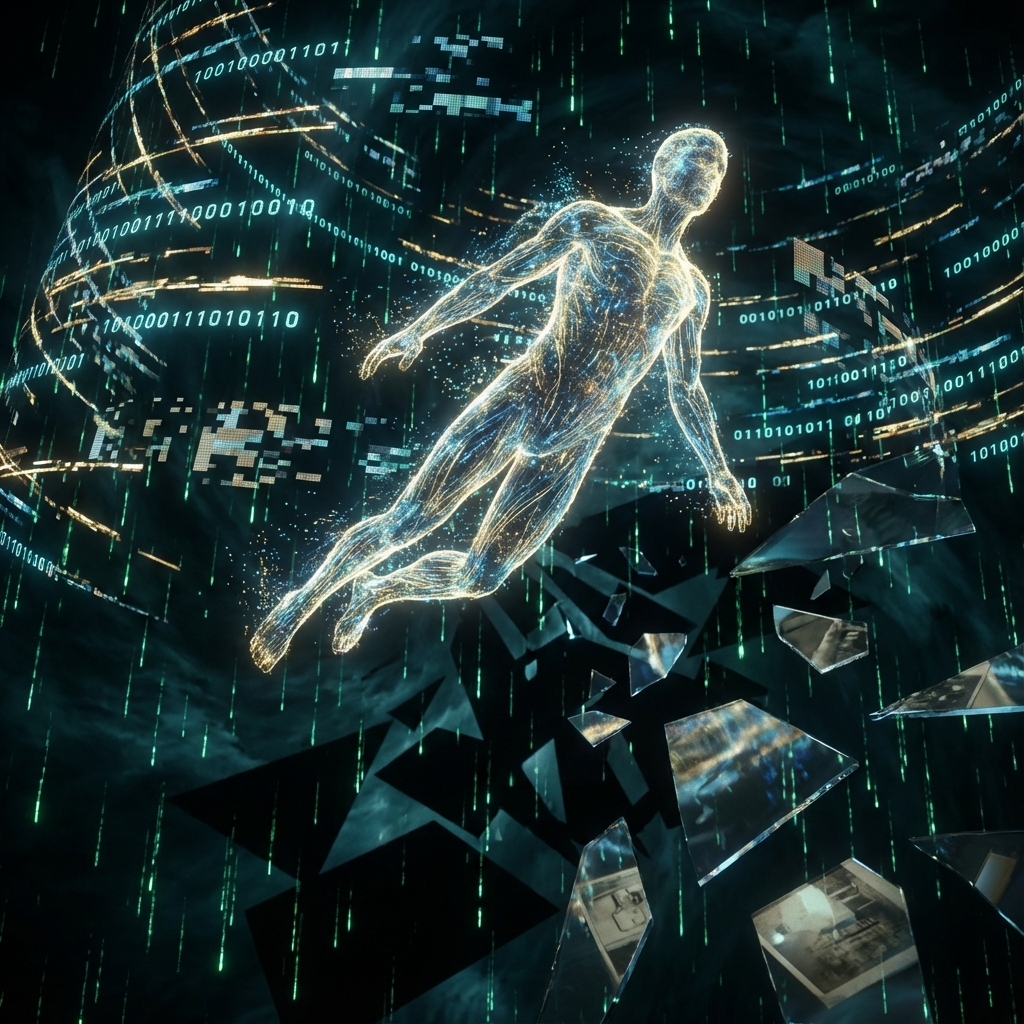
\includegraphics[height=\figheight]{Fig4-2.png}
\caption{Light-composed figure in data storm—symbolic representation of fragmented memory \\ \authorcreated}
\label{fig:light-figure}
\index{figure!symbolic avatar}
\end{figure}

This isn't spectacle, but poetic language. Through this method, creators can split the self into multiple symbolic bodies: a younger you, a digitized you, an idealized you. Each avatar is a dimension of thought.

The use of avatars helps:

\begin{itemize}
\item \textbf{Express abstract themes}\index{abstract themes}: Such as time, memory, consciousness, desire.
\item \textbf{Protect privacy}\index{privacy protection}: Making characters concrete yet not personal.
\item \textbf{Form visual style}\index{visual style}: Symbolized characters can create consistency across a series of works.
\end{itemize}

This method is widely used in brand short films and philosophical imagery, enabling AI imagery to transcend ``realism'' and move toward ``surrealism.''\index{surrealism} From our practical experience with AI-generated content, we can observe how systematic visual symbolism creates meaningful narrative structures that resonate with audiences across different cultural contexts.

\section{Brand Cameos: The Materialization of Trust}
\label{sec:brand-cameos}
\index{brand cameos}
\index{trust visualization}

In commercial narratives, cameos become a brand language. When founders, designers, or spokespersons appear in authentic or avatar form, they represent not only individuals but the spiritual essence of the brand.

For example:

\begin{Prompt}
``@samma stands beside a silver electric vehicle, light coming from the side, she smiles and points to the car's streamlined body—calm, confident, assured.''
\end{Prompt}

\begin{figure}[H]
\centering

\includegraphics[height=\figheight]{Fig4-3.png}
\caption{Brand spokesperson with product—professional yet warm atmosphere \\ \authorcreated}
\label{fig:brand-cameo}
\index{figure!brand cameo}
\end{figure}

The tone of this scene is professional yet warm. AI adjusts shot color temperature, light softness, and action stability through adjectives, allowing ``brand aura''\index{brand aura} to emerge naturally. Overly deliberate exaggeration destroys authenticity, while perfectly measured restraint enhances trust.

The core of brand cameos isn't ``promotion'' but ``humanization.''\index{humanization in branding} Audiences trust the people in the frame, not the products. The human essence of a brand thereby becomes accessible to audiences.

\section{Character Continuity: Maintaining Consistency Across Shots}
\label{sec:continuity-magic}
\index{continuity}
\index{character persistence}

One of Sora 2's most astonishing features is its ability to ``remember people.''\index{memory!character} When you introduce an @ character in the first act, the system retains their appearance, clothing, posture, and emotional baseline, allowing continuous appearance in subsequent scenes. This means—you can construct ``long-take narratives''\index{long-take narrative} through language alone.

For example:

\begin{enumerate}
\item @yuki watches snowflakes fall through the train window.
\item She disembarks; city lights flicker in her eyes.
\item She looks up, sees a familiar street corner, lips curving slightly.
\end{enumerate}

This is AI cinema's three-act continuity. Linguistic coherence achieves visual consistency. Sora 2's shot logic automatically coordinates emotional extension, making each appearance feel like a continuation of life.

\section{Emotional Echoes: When Characters Reappear}
\label{sec:emotional-echoes}
\index{emotional echoes}
\index{repetition in narrative}

The most moving narratives often aren't about ``the first time'' but ``once again.'' Repetition is the echo of emotion, allowing audiences to feel the flow of time and the arc of destiny.

\begin{Prompt}
``Years later, @sama walks into that library again. The light has grown colder, the bookshelves remain the same; he reaches out and touches that yellowed notebook.''
\end{Prompt}

\begin{figure}[H]
\centering
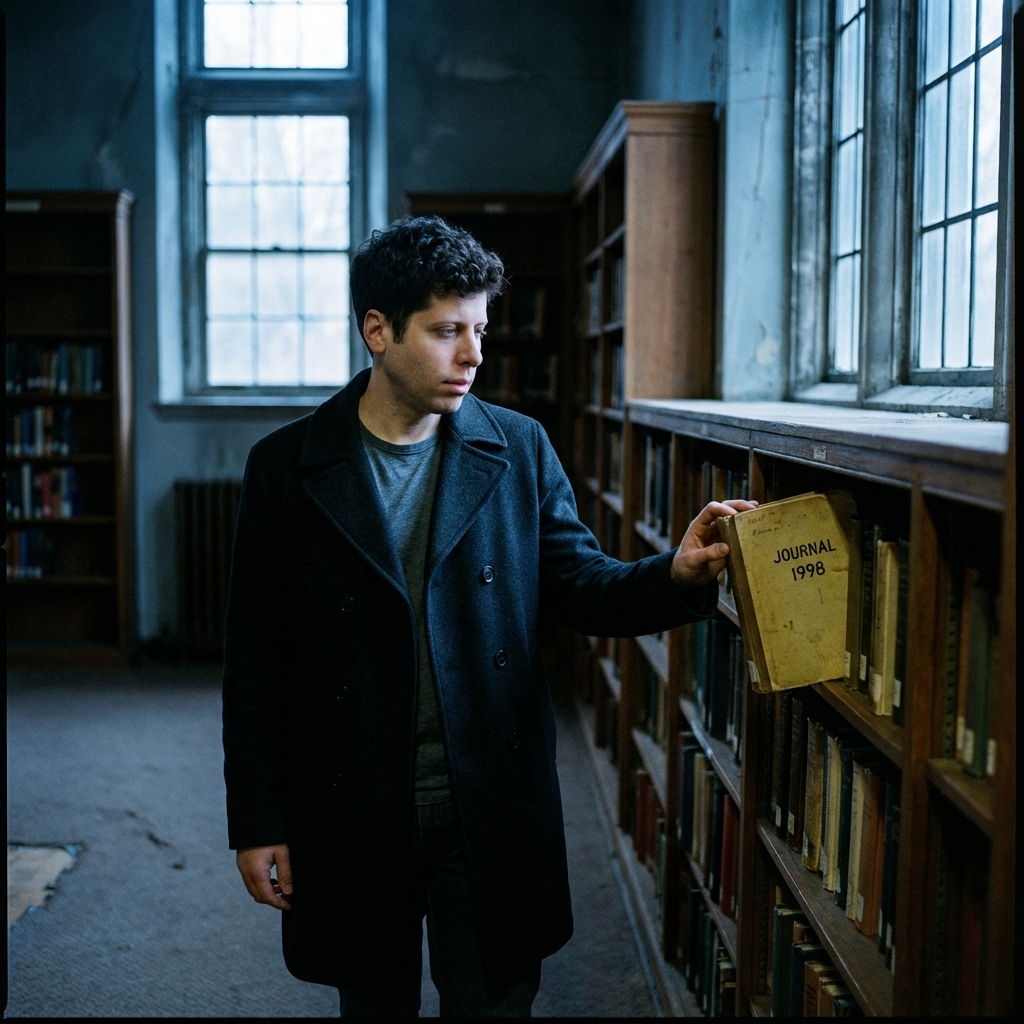
\includegraphics[height=\figheight]{Fig4-4.png}
\caption{Return to familiar place—temporal echo through visual continuity \\ \authorcreated}
\label{fig:emotional-echo}
\index{figure!temporal echo}
\end{figure}

This isn't replication but rebirth. Sora 2 can match the visual characteristics of earlier shots, creating nostalgic contrast in new scenes—that's the most human aspect of AI narrative: the temperature of time\index{temperature of time}.

\section{Conclusion: Character Integration as Narrative Foundation}
\label{sec:cameo-conclusion}
\index{cameos!conclusion}

AI's greatness lies not in algorithms but in making us reconsider the meaning of ``appearing.'' Each cameo is a declaration of ``I am here.''\index{declaration of presence} It brings creators from backstage to center stage, transforms stories from concepts to emotions.

In Sora 2's cinematic language, cameos aren't accessories but essential structural elements. They provide imagery with human context and give stories emotional resonance. The next time you write ``@someone,'' remember—it's not just a command, but a strategic narrative choice. You're integrating character presence into your visual story.

\section{Practical Guide: How to Direct Cameos in Sora 2}
\label{sec:cameo-practical-guide}
\index{cameo!practical guide}

\subsection{Step-by-Step Cameo Implementation}

\textbf{Step 1: Character Registration}
\begin{itemize}
\item Upload 3-5 clear photos from different angles
\item Provide basic descriptors: age, style, distinctive features
\item Test with simple Prompts: ``@username standing in natural light''
\end{itemize}

\textbf{Step 2: Contextual Integration}
\begin{itemize}
\item Start with environmental context: ``@username in a modern coffee shop''
\item Add emotional layer: ``@username looking thoughtful while reading''
\item Include cinematic elements: ``close-up of @username, soft lighting, shallow depth of field''
\end{itemize}

\textbf{Step 3: Performance Direction}
\begin{itemize}
\item Specify actions: ``@username slowly turns toward the camera''
\item Define expressions: ``@username smiles with a hint of melancholy''
\item Control pacing: ``@username pauses, then continues walking''
\end{itemize}

\textbf{Step 4: Continuity Management}
\begin{itemize}
\item Maintain consistent lighting and styling across shots
\item Use reference phrases: ``same outfit as previous scene''
\item Create visual callbacks: ``@username returns to the same location''
\end{itemize}

\section*{Practical Exercises}
\index{practical exercises}

\begin{quote}
\textit{\textbf{Timeless Principle:} Even as interfaces evolve and platforms update, the underlying visual logic---light, composition, rhythm, and emotional resonance---remains eternal. Master these fundamentals, and you will adapt effortlessly to any future tool.}
\end{quote}

\subsection*{Exercise 1: Cameo Setup and Testing}
\textbf{Objective}: Master the complete cameo registration and validation process.

\textbf{Registration Checklist}:
\begin{enumerate}
\item \textbf{Recording Preparation}:
   \begin{itemize}
   \item Choose well-lit, quiet environment
   \item Wear neutral clothing (avoid patterns/logos)
   \item Prepare 3-5 different expressions (neutral, happy, thoughtful, surprised)
   \item Practice clear speech at normal pace
   \end{itemize}
\item \textbf{Multi-Angle Capture}:
   \begin{itemize}
   \item Front-facing: Direct eye contact, shoulders visible
   \item Profile: Clean side view, good lighting
   \item Three-quarter: Slight angle, natural pose
   \end{itemize}
\item \textbf{Voice Sample Recording}:
   \begin{itemize}
   \item Read provided text naturally
   \item Include emotional variations (excited, calm, serious)
   \item Ensure clear pronunciation and consistent volume
   \end{itemize}
\end{enumerate}

\textbf{Testing Protocol}:
\begin{Prompt}
Start with simple Prompts:\\
"@username sitting in a chair, looking at camera"\\
"@username walking slowly, natural lighting"\\
"@username speaking to camera, friendly expression"
\end{Prompt}

\subsection*{Exercise 2: Character Direction Techniques}
\textbf{Objective}: Learn precise character direction and performance control.

\textbf{Expression Direction Practice}:
\begin{itemize}
\item \textbf{Subtle Emotions}: "@username with a slight smile, eyes showing warmth"
\item \textbf{Complex States}: "@username looking conflicted, eyebrows slightly furrowed, hesitant expression"
\item \textbf{Dynamic Changes}: "@username's expression shifts from confusion to understanding"
\end{itemize}

\textbf{Action Choreography}:
\begin{enumerate}
\item \textbf{Simple Actions}: "@username picks up coffee cup, takes a sip"
\item \textbf{Emotional Actions}: "@username nervously adjusts hair, looks away"
\item \textbf{Narrative Actions}: "@username discovers something surprising, eyes widen"
\end{enumerate}

\textbf{Practice Assignment}: Create direction Prompts for these scenarios:
\begin{itemize}
\item Character receiving good news
\item Character making a difficult decision
\item Character remembering something important
\end{itemize}

\subsection*{Exercise 3: Continuity and Consistency}
\textbf{Objective}: Maintain character consistency across multiple scenes.

\textbf{Continuity Elements}:
\begin{itemize}
\item \textbf{Wardrobe}: "same blue sweater as previous scene"
\item \textbf{Lighting}: "consistent soft lighting from left side"
\item \textbf{Mood}: "maintaining thoughtful demeanor from earlier"
\item \textbf{Location}: "returning to the same café setting"
\end{itemize}

\textbf{Multi-Scene Exercise}:
Create a three-scene sequence:
\begin{enumerate}
\item Scene 1: "@username enters café, looks around curiously"
\item Scene 2: "@username at table, same outfit, reading book intently"
\item Scene 3: "@username leaving café, same lighting, satisfied expression"
\end{enumerate}

\section*{Cameo Direction Templates}
\index{cameo templates}

\subsection*{Template 1: Character Introduction}
\begin{Prompt}
\textbf{[@username]} + [Setting/Environment] + [Initial Action] + [Emotional State] + [Camera Approach]

Example: "@sarah in modern office, organizing papers, focused concentration, medium shot with natural lighting"
\end{Prompt}

\subsection*{Template 2: Emotional Transition}
\begin{Prompt}
\textbf{[@username]} + [Starting Emotion] + [Trigger/Catalyst] + [Emotional Journey] + [Final State]

Example: "@john looking worried, receives phone call, expression gradually relaxes, ends with relieved smile"
\end{Prompt}

\subsection*{Template 3: Narrative Interaction}
\begin{Prompt}
\textbf{[@username]} + [Interaction Type] + [Response/Reaction] + [Physical Action] + [Emotional Subtext]

Example: "@maria listening to friend, nodding thoughtfully, leans forward with interest, shows genuine empathy"
\end{Prompt}

\section*{Cameo Quality Control}
\index{quality control}

\subsection*{Pre-Generation Checklist}
\begin{itemize}
\item[$\square$] \textbf{Character Reference}: Is @username properly tagged in Prompt?
\item[$\square$] \textbf{Action Clarity}: Are character actions specific and achievable?
\item[$\square$] \textbf{Emotional Direction}: Is the desired emotional state clearly described?
\item[$\square$] \textbf{Environmental Context}: Does the setting support the character action?
\item[$\square$] \textbf{Continuity Elements}: Are consistent details maintained from previous scenes?
\item[$\square$] \textbf{Technical Feasibility}: Are lighting and camera angles realistic?
\end{itemize}

\subsection*{Post-Generation Evaluation}
\begin{itemize}
\item[$\square$] \textbf{Likeness Accuracy}: Does the generated character resemble the cameo?
\item[$\square$] \textbf{Expression Match}: Do facial expressions match the Prompt direction?
\item[$\square$] \textbf{Action Execution}: Are the directed actions performed correctly?
\item[$\square$] \textbf{Voice Synchronization}: Does the voice match the character's appearance?
\item[$\square$] \textbf{Emotional Authenticity}: Do emotions appear natural and believable?
\end{itemize}

\section*{Common Cameo Challenges and Solutions}
\index{troubleshooting}

\begin{table}[H]
\centering
\caption{Cameo Direction Issues and Fixes \\ \authorillustration}
\label{tab:cameo-issues}
\begin{tabular}{p{4cm}p{4cm}p{5cm}}
\hline
\textbf{Issue} & \textbf{Symptom} & \textbf{Solution} \\
\hline
Inconsistent Appearance & Character looks different between scenes & Add "same appearance as previous scene" or specific physical descriptors \\
\hline
Unnatural Expressions & Forced or artificial facial expressions & Use more subtle emotional direction, avoid extreme expressions \\
\hline
Poor Voice Match & Voice doesn't match character or scene & Re-record cameo with better audio quality, adjust emotional tone in Prompt \\
\hline
Action Misinterpretation & Character performs wrong or unclear actions & Break complex actions into simpler steps, use more specific verbs \\
\hline
Lighting Inconsistency & Character lighting doesn't match environment & Specify lighting direction and quality in Prompt \\
\hline
\end{tabular}
\end{table}

\section*{Advanced Cameo Techniques}
\index{advanced techniques}

\subsection*{Technique 1: Emotional Layering}
Create complex emotional states by combining multiple feelings:
\begin{Prompt}
"@username showing excitement mixed with nervousness, fidgeting with anticipation while trying to appear calm"
\end{Prompt}

\subsection*{Technique 2: Temporal Character Development}
Show character growth across scenes:
\begin{Prompt}
Scene 1: "@username uncertain and hesitant"\\
Scene 2: "@username gaining confidence"\\
Scene 3: "@username fully assured and decisive"
\end{Prompt}

\subsection*{Technique 3: Interactive Storytelling}
Create characters that respond to their environment:
\begin{Prompt}
"@username reacts to off-screen sound, turns head with curiosity, then smiles with recognition"
\end{Prompt}

\section*{Chapter Summary}

Key actionable insights for cameo direction:

\begin{itemize}
\item \textbf{Character Registration}: Upload multiple angles and test with simple Prompts before complex scenes
\item \textbf{Emotional Anchoring}: Use cameos to create audience connection points and narrative focus
\item \textbf{Performance Specificity}: Direct actions, expressions, and pacing with precise language
\item \textbf{Visual Continuity}: Maintain consistent character appearance across multiple shots and scenes
\item \textbf{Temporal Storytelling}: Use character repetition and callbacks to create narrative depth and emotional resonance
\end{itemize}
